% =============================================================================
%  Data engineering report — Project 4: real-time EV charger supervision (EN)
%  Build: latexmk -xelatex report-en.tex
% =============================================================================
\documentclass[11pt, a4paper, oneside, headings=normal, numbers=noenddot, DIV=12]{scrartcl}
\usepackage[english]{babel}
\usepackage{report-style}
\graphicspath{{../livraison/figures/en/}}
\sisetup{locale=UK, group-minimum-digits=4, group-separator={,}}

\newcommand{\ReportAuthor}{LUMU BAMANA MANASSE}
\newcommand{\ReportAuthorRole}{Data engineer}
\newcommand{\ReportShortTitle}{Charger supervision · Data engineering report}
\newcommand{\ReportFooter}{October 2026 · v1.0.0}
\newcommand{\ReportKicker}{Data engineering report · Project 4}
\newcommand{\ReportTitle}{A failure detected\\within seconds}
\newcommand{\ReportSubtitle}{Real-time supervision of EV chargers:\\Kafka, Spark Structured Streaming, Iceberg, Grafana and Terraform}
\newcommand{\ReportMeta}{%
  \begin{tabularx}{\linewidth}{@{}>{\bfseries}l@{\hspace{1em}}Y@{}}
  Date & October 2026 \\
  Version & 1.0.0 (delivered and accepted) \\
  Client & Lumio Recharge (fictional company) · Engagement LUM-2026-002 \\
  GitHub repository & \url{https://github.com/MediJr/ev-charging-realtime-streaming} \\
  Language & English · \textit{version française disponible dans le dépôt}
  \end{tabularx}}
\newcommand{\ReportScenario}{Fictional scenario, simulated chargers, real carbon data: the client company and its contacts are invented to simulate
  a complete professional engagement; charger measurements come from a simulator. Carbon intensity is RTE's real-time éCO2mix data (Open Data
  Réseaux Énergies, French Open Licence). This project is not commissioned, endorsed or affiliated with RTE.}
\hypersetup{pdftitle={A failure detected within seconds: data engineering report}, pdfauthor={Lumu Bamana Manasse},
  pdfsubject={Kafka, Spark streaming, Iceberg, Grafana, Terraform, portfolio project}, pdflang={en-GB}}

\begin{document}
\sloppy
\MakeTitlePage

% =============================================================================
\section*{Document information}
\addcontentsline{toc}{section}{Document information}

\begin{tabularx}{\linewidth}{@{}>{\bfseries\sffamily}L{4.2cm}Y@{}}
\toprule
Project & Portfolio project 4: streaming, lakehouse and infrastructure as code \\
Engagement & LUM-2026-002: ``Know within seconds that a charger is failing'' \\
Client & Lumio Recharge, operator of 1,200 chargers (fictional), attention of Sophie Bernard and Karim Haddad \\
Author & Lumu Bamana Manasse, data engineer \\
Period & October 2026 \\
Data & 200 simulated chargers (one measure every 5 s); real RTE carbon intensity \\
Status & \pill{good}{DELIVERED} \pill{good}{ACCEPTED} \\
Source code & \url{https://github.com/MediJr/ev-charging-realtime-streaming} \\
\bottomrule
\end{tabularx}

\subsection*{Version history}
\begin{tabularx}{\linewidth}{@{}l l Y@{}}
\toprule
\textbf{Version} & \textbf{Date} & \textbf{Purpose} \\
\midrule
0.1 & 2026-10-26 & Scoping: brief, meeting minutes, statement of work \\
0.5 & 2026-10-26 & Streaming platform, lakehouse, supervision, Terraform \\
0.9 & 2026-10-27 & 31-hour endurance run: two defects fixed \\
1.0.0 & 2026-10-27 & Acceptance (crash, load, catch-up), final report (French and English) \\
\bottomrule
\end{tabularx}

\subsection*{Reading guide}
\begin{tabularx}{\linewidth}{@{}>{\bfseries}L{4.2cm}Y@{}}
Operations management & \hyperref[sec:summary]{1. Executive summary} and \hyperref[sec:results]{10. Results} \\
IT (cloud move) & 4. Architecture, 8. GCP infrastructure, 12. Roadmap \\
Engineer taking over & 5. Processing, 6. Lakehouse, 9. Acceptance, 11. Lessons learned \\
\end{tabularx}

\begingroup
\addtokomafont{sectionentry}{\color{primary}}
\setcounter{tocdepth}{2}
\tableofcontents
\endgroup
\clearpage

% =============================================================================
\section{Executive summary}\label{sec:summary}

\textbf{The need.} Lumio Recharge learns that a charger is down when a customer calls, sometimes hours later. Its chargers already send their
power every 5 seconds. Operations want an alert \textbf{within 30 seconds}, the \textbf{live CO\textsubscript{2} of each charging session}, and a
supervision screen. The IT department plans to move to Google Cloud next year.

\textbf{The solution.} A \textbf{streaming} platform started with a single \texttt{docker compose up}. Measures flow through a
\textbf{Kafka}-compatible event log (Redpanda), are processed in \textbf{event time} by \textbf{Spark Structured Streaming} (watermark,
deduplication, per-charger state), kept in an \textbf{Apache Iceberg lakehouse}, enriched with RTE's \textbf{real} carbon intensity, and shown in
\textbf{Grafana}. The target Google Cloud infrastructure is written in \textbf{Terraform}.

\kpirow{27 / 27}{anomalies\\detected}{11.6 s}{detection delay\\at the 95\textsuperscript{th} percentile}{0}{false\\alert}{0}{message lost or doubled\\after a hard kill}
\kpirow{83,292}{messages reconciled\\one by one}{8.4 s}{to catch up\\3,654 messages}{≈ 1,440}{messages/s\\(measured capacity)}{22}{tests, 5 of them\\Spark end to end}

\begin{keybox}[Key takeaways]
\begin{itemize}[leftmargin=1.2em]
  \item \textbf{Q1 · Delay:} all 27 injected anomalies detected in 5.9 s (median) and 11.6 s (95\textsuperscript{th} percentile). Target: 30 s.
  \item \textbf{Q2 · Anomalies:} silent charger, overpower, stuck charger, each opened then resolved, without an alert storm.
  \item \textbf{Q3 · CO\textsubscript{2}:} 186 sessions, 4.8 MWh, 211 kg of CO\textsubscript{2} at that evening's real RTE intensity (44 g/kWh).
  \item \textbf{Q4 · Robustness:} Spark killed mid-stream, resumed with no loss and no duplicate. Capacity of about 1,440 messages/s, i.e.
        some 7,000 chargers: six times the current fleet.
\end{itemize}
\end{keybox}

\textbf{Three defects were found by running the platform for real} (31-hour endurance, crash, overload), fixed and covered by tests: an empty
timestamp column rejected by Arrow, measure identifiers repeating after a restart, and silent chargers missed during a catch-up.

% =============================================================================
\section{Context and scoping}

\begin{table}[H]
\centering\small
\begin{tabularx}{\linewidth}{@{}L{5.8cm} Y@{}}
\toprule
\textbf{Client request} & \textbf{Technical consequence} \\
\midrule
``Detect within seconds'' & \textbf{Continuous} processing (streaming), not batches \\
``A charger that stops answering'' & Detect an \textbf{absence} of events: per-charger state and timeout \\
4G network delaying or duplicating messages & \textbf{Event time}, watermark, deduplication \\
``Move to Google Cloud without a rewrite'' & Open formats (Iceberg), Kafka API, infrastructure in \textbf{Terraform} \\
A crash must lose or double nothing & Checkpoints, idempotent writes \\
\bottomrule
\end{tabularx}
\caption{From request to technical requirements}
\end{table}

\begin{table}[H]
\centering\small
\begin{tabularx}{\linewidth}{@{}L{3.3cm} Y L{2.3cm}@{}}
\toprule
\textbf{Anomaly} & \textbf{Rule (scoping)} & \textbf{Severity} \\
\midrule
Silent charger & No message for more than 60 s & critical \\
Overpower & Power above 110\% of the rated power & high \\
Stuck charger & Open session at 0 kW for more than 2 minutes & medium \\
\bottomrule
\end{tabularx}
\caption{The three anomalies and their rules}
\end{table}

% =============================================================================
\section{Data}

\textbf{Charger measures (simulated).} 200 chargers on 12 sites, two thirds at 22 kW and one third at 50 kW, one measure every 5 s: power,
session energy, status, current session. The simulator \textbf{deliberately} injects faults, and publishes each injection to a
\textbf{ground-truth} topic (\texttt{sim.injections}) used to check every detection.

\begin{table}[H]
\centering\small
\begin{tabularx}{\linewidth}{@{}L{4.4cm} L{3.2cm} Y@{}}
\toprule
\textbf{Injected fault} & \textbf{Frequency} & \textbf{What it tests} \\
\midrule
Silent, overpower, stuck charger & ≈ 0.3 per charger per hour & The three anomaly rules \\
Duplicate message & 1\% & Deduplication \\
Delay of 5 to 40 s & 1\% & Event time \\
Delay of 3 to 5 min & 0.2\% & Watermark: dropped and counted \\
\bottomrule
\end{tabularx}
\caption{Faults injected by the simulator (ADR 005)}
\end{table}

\textbf{Carbon intensity (real).} A collector reads RTE's real-time éCO2mix API every 5 minutes, the same source as project 2, and publishes
each 15-minute slot to a \textbf{compacted} topic: only the latest value of each slot is kept.

% =============================================================================
\section{Architecture}

\begin{figure}[H]
\centering
\resizebox{\linewidth}{!}{%
\begin{tikzpicture}[
  font=\sffamily\small, node distance=0.6cm and 0.75cm,
  src/.style={draw=rule, fill=panel, rounded corners=2pt, minimum width=2.4cm, minimum height=1.1cm, align=center},
  stage/.style={draw=primary, fill=primary, text=white, rounded corners=3pt, minimum width=2.6cm, minimum height=1.3cm, align=center, font=\sffamily\small\bfseries},
  store/.style={cylinder, shape border rotate=90, aspect=0.18, draw=accent, fill=accent!8, minimum width=2.3cm, minimum height=1.3cm, align=center},
  arr/.style={-{Stealth[length=2.6mm]}, thick, color=ink2}]
  \node[src] (sim) {Simulator\\\scriptsize 200 chargers};
  \node[src, below=0.5cm of sim] (rte) {RTE API\\\scriptsize real-time CO\textsubscript{2}};
  \node[store, right=1.2cm of $(sim)!0.5!(rte)$] (rp) {\scriptsize Redpanda\\\scriptsize Kafka API};
  \node[stage, right=1.2cm of rp] (sp) {SPARK\\\scriptsize\mdseries event time\\\scriptsize\mdseries watermark · state};
  \node[store, right=1.6cm of sp, yshift=1.1cm] (ice) {\scriptsize Iceberg (S3)\\\scriptsize bronze·silver·gold};
  \node[store, right=1.6cm of sp, yshift=-1.1cm] (pg) {\scriptsize PostgreSQL\\\scriptsize serving};
  \node[src, right=0.9cm of pg] (gf) {Grafana\\\scriptsize 13 panels};
  \draw[arr] (sim) -- (rp); \draw[arr] (rte) -- (rp); \draw[arr] (rp) -- (sp);
  \draw[arr] (sp) -- (ice); \draw[arr] (sp) -- (pg); \draw[arr] (pg) -- (gf);
  \draw[arr, dashed] (sp.north) to[bend right=35] node[above, font=\scriptsize\sffamily, text=ink2]{charger.alerts} (rp.north);
\end{tikzpicture}}
\caption{From the charger to the supervision screen}
\end{figure}

\begin{table}[H]
\centering\small
\begin{tabularx}{\linewidth}{@{}L{3cm} L{3.6cm} Y@{}}
\toprule
\textbf{Role} & \textbf{Choice} & \textbf{Why (ADR)} \\
\midrule
Event log & Redpanda v25.3 & Kafka protocol, single binary, light; replaceable by managed Kafka (001) \\
Processing & Spark 4.0 Structured Streaming & Event time, watermark, fault-tolerant state (001) \\
Lakehouse & Iceberg 1.10 on S3, JDBC catalog & Transactions, open format read by BigQuery (002) \\
Serving & PostgreSQL 17 & Screen refresh in milliseconds (003) \\
Supervision & Grafana 12, provisioned as code & Observability standard (003) \\
Cloud & Terraform, Google provider 8.8 & Infrastructure reviewed and versioned before it exists (004) \\
\bottomrule
\end{tabularx}
\caption{Technical choices}
\end{table}

% =============================================================================
\section{Spark processing}

A single Spark application runs six queries, each with its own checkpoint:

\begin{table}[H]
\centering\small
\begin{tabularx}{\linewidth}{@{}L{2.2cm} L{1.6cm} Y L{3.4cm}@{}}
\toprule
\textbf{Query} & \textbf{Trigger} & \textbf{Processing} & \textbf{Destination} \\
\midrule
bronze & 30 s & None: the message as received, with its Kafka position & Iceberg \\
silver & 30 s & JSON parsing, 2-minute watermark, deduplication & Iceberg \\
monitor & 5 s & Per-charger state and anomaly rules & PostgreSQL, Kafka, Iceberg \\
minutes & 30 s & Energy per charger and closed minute, CO\textsubscript{2} & PostgreSQL, Iceberg \\
grid\_co2 & 30 s & RTE carbon intensity & PostgreSQL, Iceberg \\
injections & 30 s & Simulator ground truth & PostgreSQL \\
\bottomrule
\end{tabularx}
\caption{The six continuous queries}
\end{table}

\subsection{Event time, watermark and deduplication}
A measure is placed according to the time \textbf{the charger produced it}, not when it arrived. The 2-minute \textbf{watermark} says how long
Spark waits for latecomers: beyond it, a measure is dropped, and counted in the micro-batch log. Deduplication uses the measure identifier,
\texttt{event\_id}.

\subsection{Per-charger state and detecting an absence}
The rules are written in \textbf{pure Python} (\texttt{lumio\_stream.monitor}), tested without Spark. Spark calls them for each charger with its new
measures and its stored state (\texttt{applyInPandasWithState}). A charger that sends nothing triggers nothing: a 60-second
\textbf{processing-time timeout}, reset on every measure, raises the ``silent charger'' alert.

\begin{warnbox}[Limit found during acceptance: catch-up]
When Spark catches up a backlog, it crosses several minutes of event time in a few seconds: the processing-time timeout does not fire, and 3 silent
chargers were missed. An \textbf{event-time safety net} was added: a gap of more than 60 s between two measures, noticed when the charger comes back,
opens and closes the alert. It arrives late, but is \textbf{never lost}.
\end{warnbox}

% =============================================================================
\section{Iceberg lakehouse}

\begin{table}[H]
\centering\small
\begin{tabularx}{\linewidth}{@{}L{3.6cm} L{3.2cm} Y@{}}
\toprule
\textbf{Table} & \textbf{Grain} & \textbf{Content} \\
\midrule
bronze.telemetry\_raw & one Kafka message & Raw message, Kafka partition and offset \\
silver.telemetry & one measure & Typed, deduplicated fields \\
gold.charger\_minute & charger × minute & Energy, CO\textsubscript{2} \\
gold.alerts & state change & Opened or resolved alert, anomaly and detection times \\
\bottomrule
\end{tabularx}
\caption{Lakehouse tables (partitioned by day)}
\end{table}

\textbf{Exactly once.} Spark's native Iceberg sink is exactly-once by design. For writes made in \texttt{foreachBatch}, which only guarantees
``at least once'', each append is tagged with the micro-batch id in the Iceberg snapshot: a batch replayed after a crash is skipped. Serving writes
are UPSERTs.

\textbf{Maintenance.} Streaming writes one small file per micro-batch. A daily script deletes raw measures older than 90 days, compacts small files
and expires old snapshots.

% =============================================================================
\section{Supervision}

The Grafana screen (13 panels, provisioned as code, anonymous read-only access) first shows \textbf{open alerts} sorted by severity, then chargers
online, fleet power, RTE intensity, detection delay at the 95\textsuperscript{th} percentile, throughput, ongoing sessions with their
CO\textsubscript{2}, and stream health (rows dropped by the watermark). A \texttt{StreamingQueryListener} logs every micro-batch to the serving database.

% =============================================================================
\section{Google Cloud infrastructure in Terraform}

\begin{table}[H]
\centering\small
\begin{tabularx}{\linewidth}{@{}L{4.2cm} Y@{}}
\toprule
\textbf{Resource} & \textbf{Choice} \\
\midrule
Lakehouse bucket & Paris region, public access prevented, versioning, raw measures deleted after 90 days \\
BigQuery + BigLake & Dataset for gold tables; BigLake connection to read Iceberg without copying \\
Service accounts & One per use: processing writes, supervision only reads \\
Budget alert & 50, 90 and 100\% of a monthly budget \\
\bottomrule
\end{tabularx}
\caption{Described infrastructure (ADR 004)}
\end{table}

\texttt{terraform fmt}, \texttt{init -backend=false} and \texttt{validate} pass, locally and in continuous integration. A \texttt{plan} needs GCP
credentials: it will be run with the IT department. Mapping: SeaweedFS becomes Cloud Storage, local Spark becomes Dataproc Serverless (same code),
Redpanda becomes managed Kafka (same protocol).

% =============================================================================
\section{Acceptance}

Acceptance ran on a \textbf{fresh platform}, with Spark hard-killed mid-stream, then a load test.

\begin{table}[H]
\centering\small
\begin{tabularx}{\linewidth}{@{}l Y c@{}}
\toprule
\textbf{\#} & \textbf{Criterion} & \textbf{Result} \\
\midrule
C1 & Starts with \texttt{docker compose up} on a fresh platform & \ok \\
C2 & All three injected anomaly types detected (27 / 27, 0 false alert) & \ok \\
C3 & Detection delay < 30 s at the 95\textsuperscript{th} percentile (11.6 s) & \ok \\
C4 & Duplicates counted once, latecomers counted separately & \ok \\
C5 & Spark hard kill: no loss, no duplicate & \ok \\
C6 & CO\textsubscript{2} computed with the real RTE intensity & \ok \\
C7 & Terraform validated, tests green & \ok \\
C8 & No secret in version control & \ok \\
\bottomrule
\end{tabularx}
\caption{Acceptance criteria: 8 out of 8}
\end{table}

\subsection{Reconciliation: every message is explained}

\begin{terminal}{spark/recette.py · messages arrived before 19:46:59}
\begin{lstlisting}[style=terminal]
bronze messages             :    83,292   (distinct Kafka positions: 83,292)
distinct identifiers        :    82,484   -> duplicates dropped: 808
silver measures             :    82,347   (distinct identifiers: 82,347)
identifiers missing in silver:      137
equation: 83,292 = 82,347 + 808 + 137  -> OK
message read twice by Spark : 0
injections before the cutoff: {'too_late': 164, 'late': 882, 'duplicate': 808}
missing explained by an injected 3-5 min delay: 137 / 137
\end{lstlisting}
\end{terminal}

The 808 duplicates dropped are exactly the 808 duplicates injected. The 137 missing measures are all injected delays beyond the watermark. No Kafka
message was read twice, despite the hard kill: the first micro-batch after restart is number 41, right after batch 40 committed before the crash,
and it caught up 3,654 messages in 8.4 s.

% =============================================================================
\section{Results}\label{sec:results}

\subsection*{Q1 · Detection delay}
\begin{figure}[H]
\centering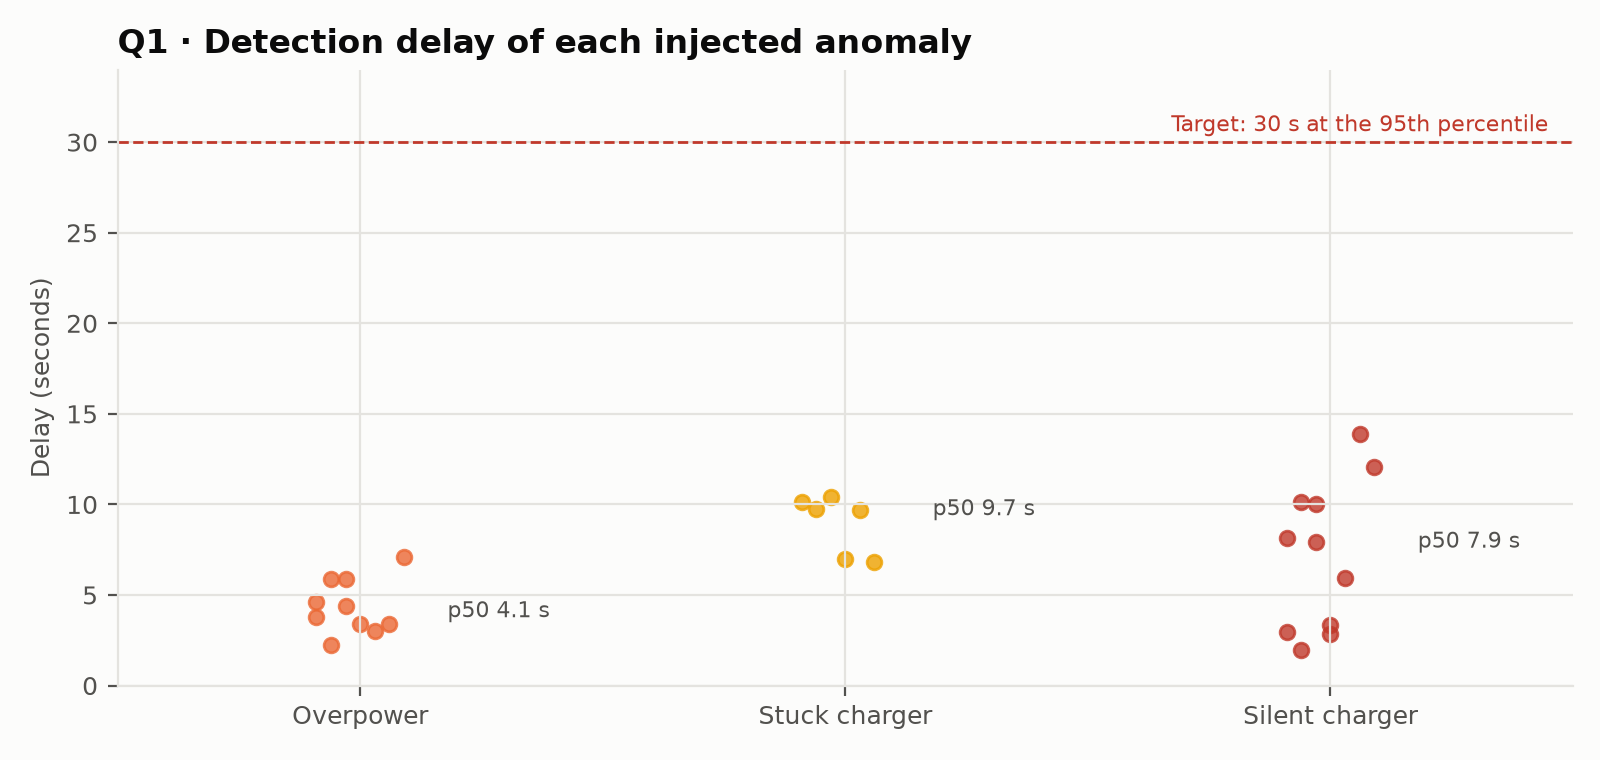
\includegraphics[width=0.86\linewidth]{q1_delai_detection.png}
\end{figure}
All 27 anomalies injected during the nominal period are detected, with no false alert: overpower in 4.1 s (median), stuck charger in 9.7 s, silent
charger in 7.9 s. The 95\textsuperscript{th} percentile is \textbf{11.6 s}, the maximum 13.9 s.

\subsection*{Q2 · Alerts by site}
\begin{figure}[H]
\centering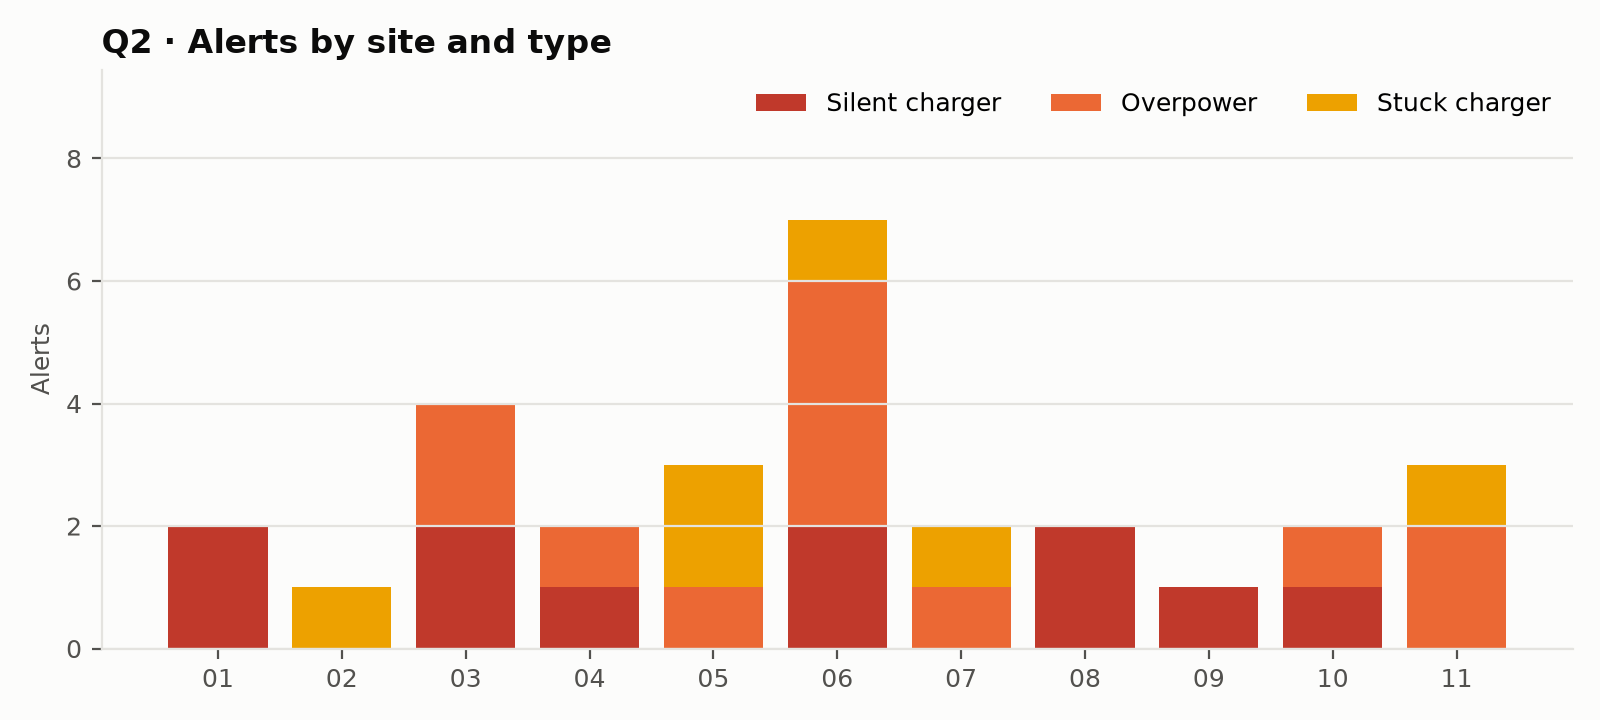
\includegraphics[width=0.86\linewidth]{q2_alertes_par_site.png}
\end{figure}

\subsection*{Q3 · CO\textsubscript{2} of charging sessions}
\begin{figure}[H]
\centering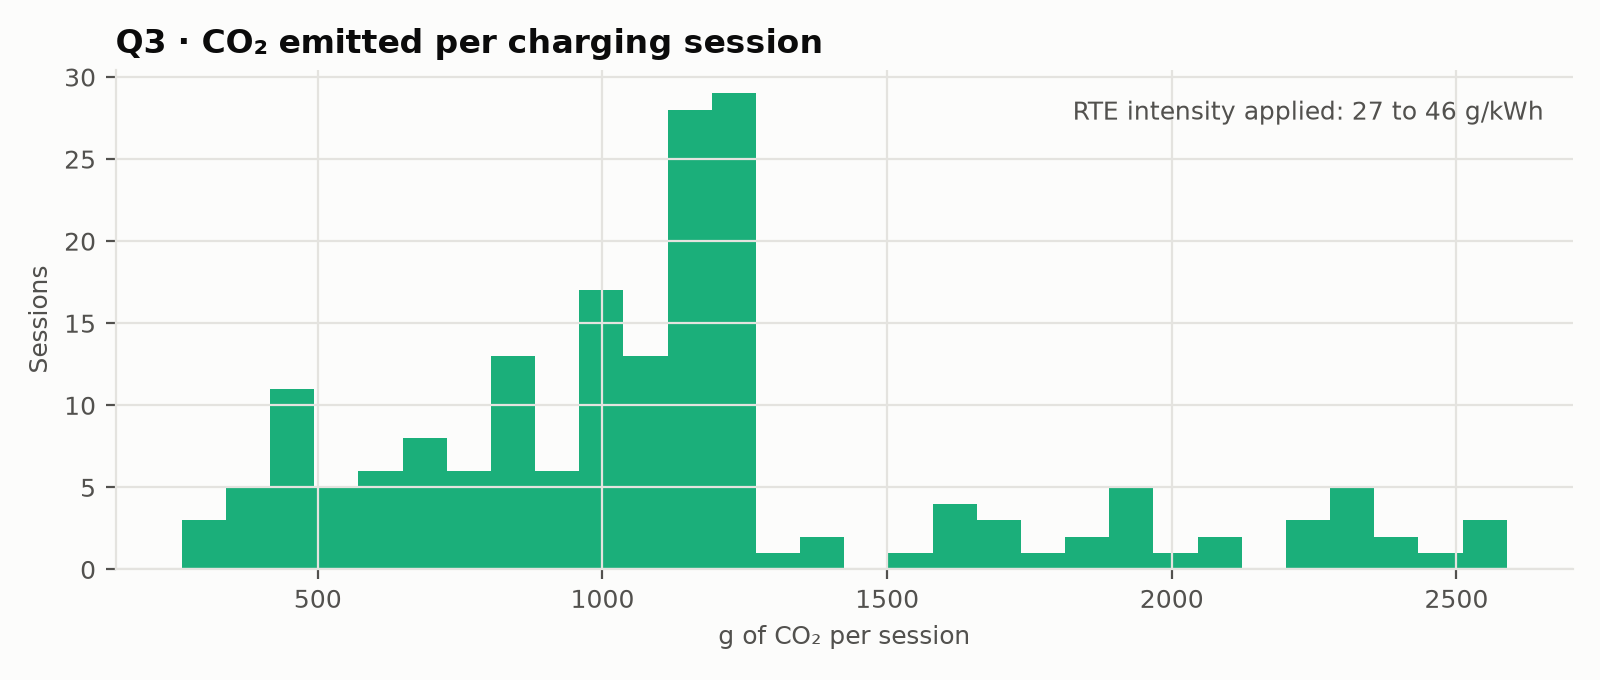
\includegraphics[width=0.86\linewidth]{q3_co2_par_recharge.png}
\end{figure}
186 sessions delivered 4.8 MWh and emitted 211 kg of CO\textsubscript{2}, at the grid's real intensity that evening (44 g/kWh on average): a median of
1.1 kg per session. The same computation is shown live for each ongoing session.

\subsection*{Q4 · Crash, catch-up and load}
\begin{figure}[H]
\centering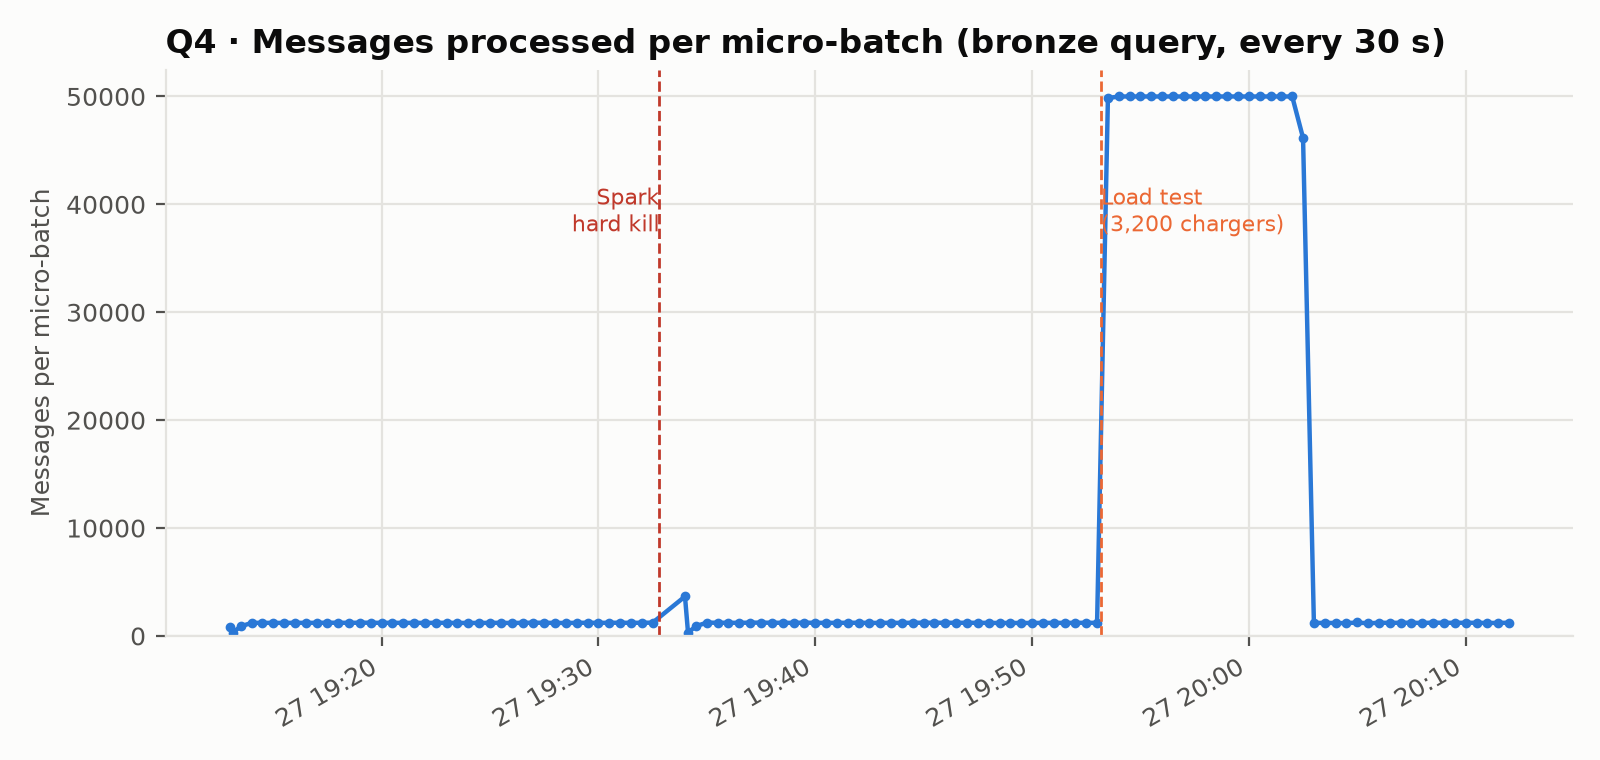
\includegraphics[width=0.86\linewidth]{q4_debit_reprise_charge.png}
\end{figure}

\begin{table}[H]
\centering\small
\begin{tabularx}{\linewidth}{@{}L{4.6cm} Y@{}}
\toprule
\textbf{Load test (≈ 2,960 messages/s)} & \textbf{Result} \\
\midrule
Bronze and silver & Keep up: up to 5,700 and 4,600 messages/s \\
Stateful monitor & \textbf{Bottleneck}: ≈ 1,440 messages/s; detection at 130-160 s during the overload \\
Stability & No crash; backlog cleared 10 minutes after the overload ended \\
Capacity & ≈ 7,000 chargers at one measure every 5 s, for a fleet of 1,200 \\
\bottomrule
\end{tabularx}
\caption{What the platform handles on a laptop}
\end{table}

% =============================================================================
\section{Lessons learned}
\begin{table}[H]
\centering\small
\begin{tabularx}{\linewidth}{@{}L{4.3cm} Y@{}}
\toprule
\textbf{Defect or incident} & \textbf{Lesson} \\
\midrule
Spark tests silently skipped & A ``skipped'' test is not a passed test: check how many tests actually ran \\
Empty timestamp column rejected by Arrow & The first real batch holds cases no example contained \\
\texttt{event\_id}s repeating after a restart & A deduplication key must be unique \textbf{over time}, not within one run \\
First reconciliation wrong & Two tables written by two queries are never at the same instant: compare a fixed set \\
Silent chargers missed during catch-up & A processing-time timeout makes no sense when time is ``fast-forwarded'' \\
Spark stops after laptop sleep & Checkpoints and the restart policy recovered alone; a manual \texttt{docker kill} does not \\
\bottomrule
\end{tabularx}
\caption{What this project taught}
\end{table}

% =============================================================================
\section{Roadmap}
\begin{enumerate}[leftmargin=1.4em]
  \item \textbf{Capacity}: monitor in Scala (\texttt{transformWithState}) or a Dataproc cluster, more Kafka partitions.
  \item \textbf{Outgoing alerts}: a \texttt{charger.alerts} consumer to SMS and ticketing, with deduplication.
  \item \textbf{GCP deployment}: \texttt{terraform plan} with the IT department, then Dataproc Serverless and managed Kafka.
  \item \textbf{Real chargers}: an OCPP gateway to the \texttt{charger.telemetry} topic, with no change to the processing.
\end{enumerate}

\end{document}
